\section{Design und Entwicklung des Gehäuses}
Die Entwicklung eines Geräts umfasst in der Regel mehrere Schritte, beginnend mit der Entwurfsphase. In dieser Phase ist zunächst eine Entscheidung darüber zu treffen, wie das Gerät angesichts der Anforderungen, die gestellt werden, aussehen soll. Die Anforderung, 21 Kammern zu haben, ist in diesem Kontext von besonderem Interesse, da sie die Gestaltungsmöglichkeiten erheblich einschränkt. Allerdings ist diese Einschränkung positiv zu bewerten, da die Anforderungen für die ersten Schritte als zu gering empfunden werden. Es bestehen keine Anforderungen an die physischen Beschaffenheit des Geräts, wie etwa die Größe oder das Gewicht. Dies eröffnet einen bemerkenswert großen Gestaltungsspielraum hinsichtlich der äußeren Erscheinung des Geräts.

Es gibt also schon erste Ideen, wie das Gerät aussehen soll, jede mit ihren eigenen Vor- und Nachteilen. Hier geben wir einen kurzen Überblick über die möglichen Entwürfe, die uns eingefallen sind.

\subsection{Frühe Ideen}
\subsubsection{Pillendosiersystem}
Bei den Überlegungen, wie die Pillen ausgegeben werden sollen, sind einige Ideen entstanden, die von der Umgebung inspiriert sind. Im Folgenden finden Sie kurze Beschreibungen der Systeme und auch ein Bild \ref{fig:designs} der Entwürfe, wie sie aussehen würden. Bitte beachten Sie, dass ich hier nicht zu sehr ins Detail gehe, da sie das Ergebnis eines Brainstormings waren und ich am Ende eine Idee als primäres System ausgewählt habe, aber einige Ansätze aus den anderen Ideen für das große Design übernommen habe.
\begin{itemize}
	\item  Das \textbf{Revolver}-System war das einfachste, und es dauerte nicht lange, zu diesen Idee zu kommen, denn solche Geräte wurden bereits entwickelt\cite{LiveFinePillDispenser}. Seine Vorteile sind die Einfachheit des Mechanismus, die Robustheit und der niedrige Preis, während ein Nachteil seine Größe ist und er einen Motor benötigt, um ein ziemlich großes Rad anzutreiben.
	\item Der zweite Entwurf ist der des \textbf{Karussells}. Die Hauptidee ist, dass es viel kleiner ist und den Raum effizienter nutzt als das Revolversystem. Die kleineren Räder würden sich mit einer geringeren Geschwindigkeit drehen als der Hauptarm, der sie hält, da sie mit einem Untersetzungsgetriebe und einem Riemen an der Hauptachse befestigt sind. Obwohl es geringfügig platzsparender ist als ein Revolversystem, ist es viel komplexer und benötigt immer noch einen Motor, um die gesamte Struktur zu steuern.
	\item Der dritte Entwurf ist der des \textbf{Förderbandes}. Auf dem Bild \ref{fig:designs} kann man sehen, dass es rund ist, es könnte jedoch theoretisch auch elliptisch oder mit anderen, gewundeneren Kurven gestaltet werden. Das Prinzip ist wie folgt: An dem Band ist eine Ausgabekammer angebracht, die eine Reihe dieser Kammern auf einem bestimmten Weg bewegt. Es ähnelt dem Revolversystem, aber die Kammern wären abnehmbar und das Förderband würde eine gewisse Flexibilität bei der Konstruktion des Geräts ermöglichen. Die größten Nachteile sind die Notwendigkeit eines Motors, die Notwendigkeit eines Kammermanagementsystems und die allgemeine Komplexität des Geräts.
	\item Der vierte Entwurf ist von \textbf{Verkaufsautomaten} inspiriert. Er hätte 21 Kammern, an denen jeweils ein Elektromagnet angebracht wäre. Bei jeder Ausgabe wird der Elektromagnet aktiviert, wodurch sich die Kammer verschiebt und die Pillen auf den Ausgabebereich fallen. Bei diesem Entwurf wird der Schrittmotor überflüssig, aber die Einfachheit geht verloren, da eine logische Schaltung erforderlich ist, die 21 parallel geschaltete Kammern miteinander verbindet. Theoretisch wäre eine Parallelschaltung zwar von Vorteil, aber für uns ist das nicht der Fall, da wir sie nicht sinnvoll nutzen können.
\end{itemize}
\subsubsection{Pillenrücknahmesystem}
Die Idee für das Rücknahmesystem war damals, dass es das Abgabesystem spiegelt, indem es entweder direkt darunter positioniert wird oder so, dass die Tabletten zunächst auf eine Rampe fallen, die nach einer gewissen Zeit durch eine andere Aktion in den Rückholmechanismus befördert wird. Es ist unschwer zu erkennen, dass die Wahl des Rücknahmesystems in hohem Maße von dem von uns entwickelten Dosiersystem abhängt, weshalb eine detailliertere Beschreibung später erfolgen wird, wenn wir uns näher mit dem gewählten Dosiersystem befassen.
\begin{figure}[h]
	\centering
	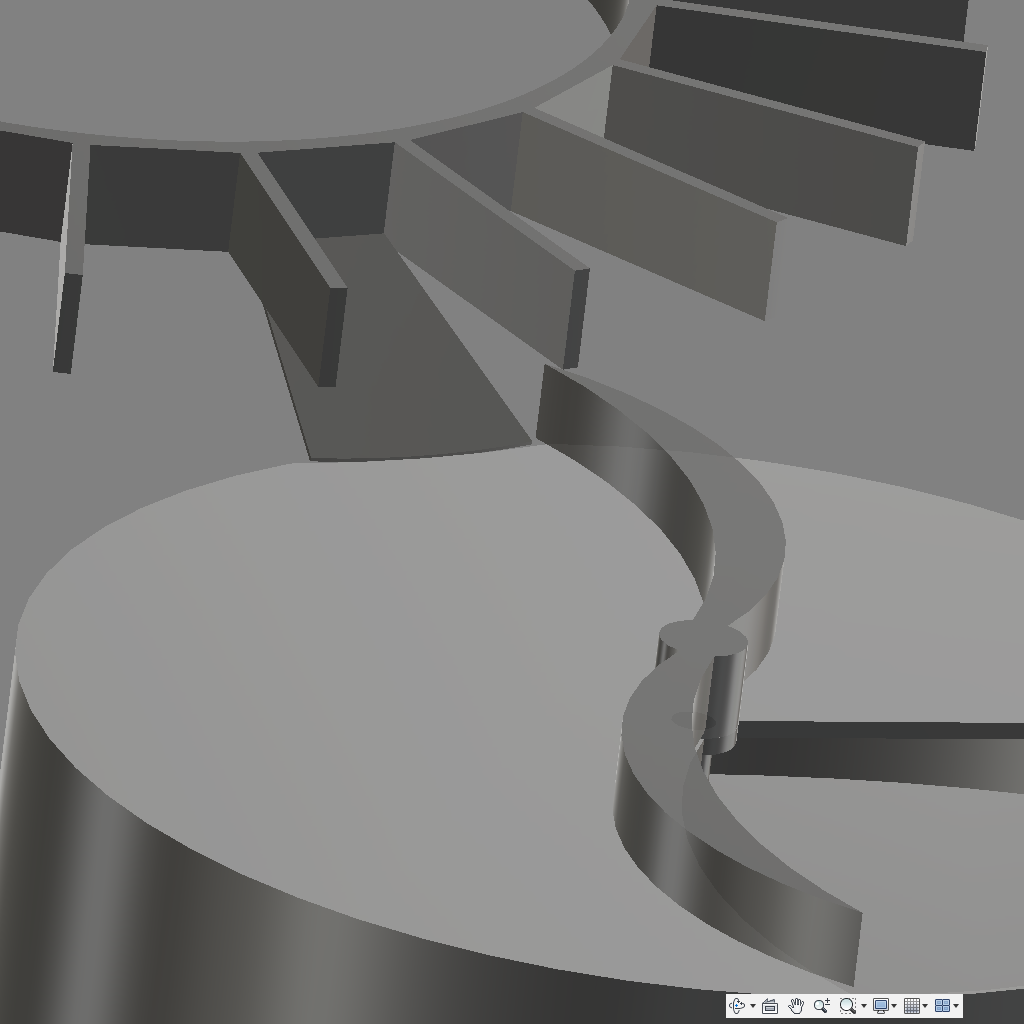
\includegraphics[width=0.7\linewidth]{Figures/Screenshot_1.png} 
	\caption[Frühe Entwürfe]{Erste Ideen, wie die Hauptstruktur (Dispenser) des Geräts aussehen soll. 1. Revolver-System. 2. Karussell-System. 3. Fördersystem (Running Sushi). 4 Automaten-System }
	\label{fig:designs}
\end{figure}
\newpage
\subsection{Auswahl des Designs}
Von allen vorgeschlagenen Entwürfen schien das Revolversystem die sinnvollste Wahl zu sein, allerdings bedurfte es einiger Verbesserungen im Design. Eine kurze Marktrecherche (z.b. \cite{LiveFinePillDispenser} \cite{zoksi_pill_organizer}) hat gezeigt, dass es nicht wirklich ein solches System gibt, das die oben genannten Anforderungen, nämlich einen Rückholmechanismus zu haben, erfüllen würde. Aus diesem Grund müsste das Design verbessert werden.
\subsubsection{Verbesserungen des Revolversystems}
Nachdem wir den Hauptmechanismus ausgewählt haben, müssen wir nun die Details ausarbeiten. Die Design-Philosophie war, es so einfach wie möglich zu machen, mit so wenig beweglichen Details. Die ersten Ideen waren in dieser Hinsicht nicht sehr erfolgreich. Auf dem Bild \ref{fig:screenshot1} können Sie sehen, wie die früheren Ideen aussehen würden. Jede Kammer hätte ihre eigene Tür, unter dieser Tür wäre eine Kerbe für den Hebel, der darin einrastet, um sie zu öffnen. Danach würden die Pillen in die Entsorgungsschale fallen. Nach einer bestimmten Zeit (15 Minuten) würde sich der S-förmige Arm drehen und die Pillen weiter die Rampe hinunter in das Entsorgungslager fallen lassen. Diese Lösung hatte zahlreiche Nachteile:
\begin{enumerate}
	\item{\textbf{Zu viele bewegliche Teile}}
	
	Jede Kammer hat 21 Türen. Die Türen brauchen einen Hebel zum Öffnen (22), dieser Hebel muss translatorisch in die Kerbe ein- und ausgerastet werden (23), der Revolvermechanismus muss sich drehen (24), der Entsorgungsarm muss sich ebenfalls drehen (25, aber die Idee war, ihn mit der Hauptachse mittels Riemen zu synchronisieren), die Entsorgungskammern müssten sich ebenfalls drehen (26). Das war zwar eine Lösung, aber angesichts der Anzahl der beweglichen Teile nicht optimal. Obwohl sich die Abgabekammern, die Entsorgungskammern und der Entsorgungsarm um dieselbe Achse drehen würden, würde das Rotation und Translation des Hebels für eine Öffnung einen komplexen Mechanismus erfordern, der die Aufwand weiter erhöht.
	\item{\textbf{Erfordert eine große Spenderschale}}
	
	Der Entsorgungsmechanismus ist an sich schon recht groß (bei diesem Prototyp wurde ein Durchmesser von 300 mm gemessen). Würde man eine weitere horizontale Fläche neben dieser Fläche hinzufügen, selbst wenn sie nur halb so groß wäre (eine Verkleinerung würde es Menschen mit motorischen Störungen erschweren, die Pillen sicher zu entnehmen), würde das gesamte System extrem groß werden.
	\item{\textbf{Enthält mehrere kleine Objekte}}
	
	Dies ist kein offensichtlicher Nachteil, aber jede Falltür muss sich um eine bestimmte Achse drehen. Diese Achse muss entweder aus einem kleinen Metallstab bestehen, der in die Öffnungen der Tür eingeführt wird, oder aus 3D-gedruckten Zähnen auf dem Design des Türs selbst. Die erste Lösung erfordert eine gewagte und präzise Montage von 21 Türen, die zweite erfordert eine hohe 3D-Druckpräzision, die auf herkömmliche Weise nicht erreicht wird.
\end{enumerate}
Aufgrund dieser Nachteile wurde das System verworfen und nie weiter verbessert. Eine wichtige Lektion wurde jedoch gelernt: Wenn wir das einfachste Design haben wollen, müssen wir uns die Kraft der Schwerkraft zu Nutze machen.
\begin{figure}[h]
	\centering
	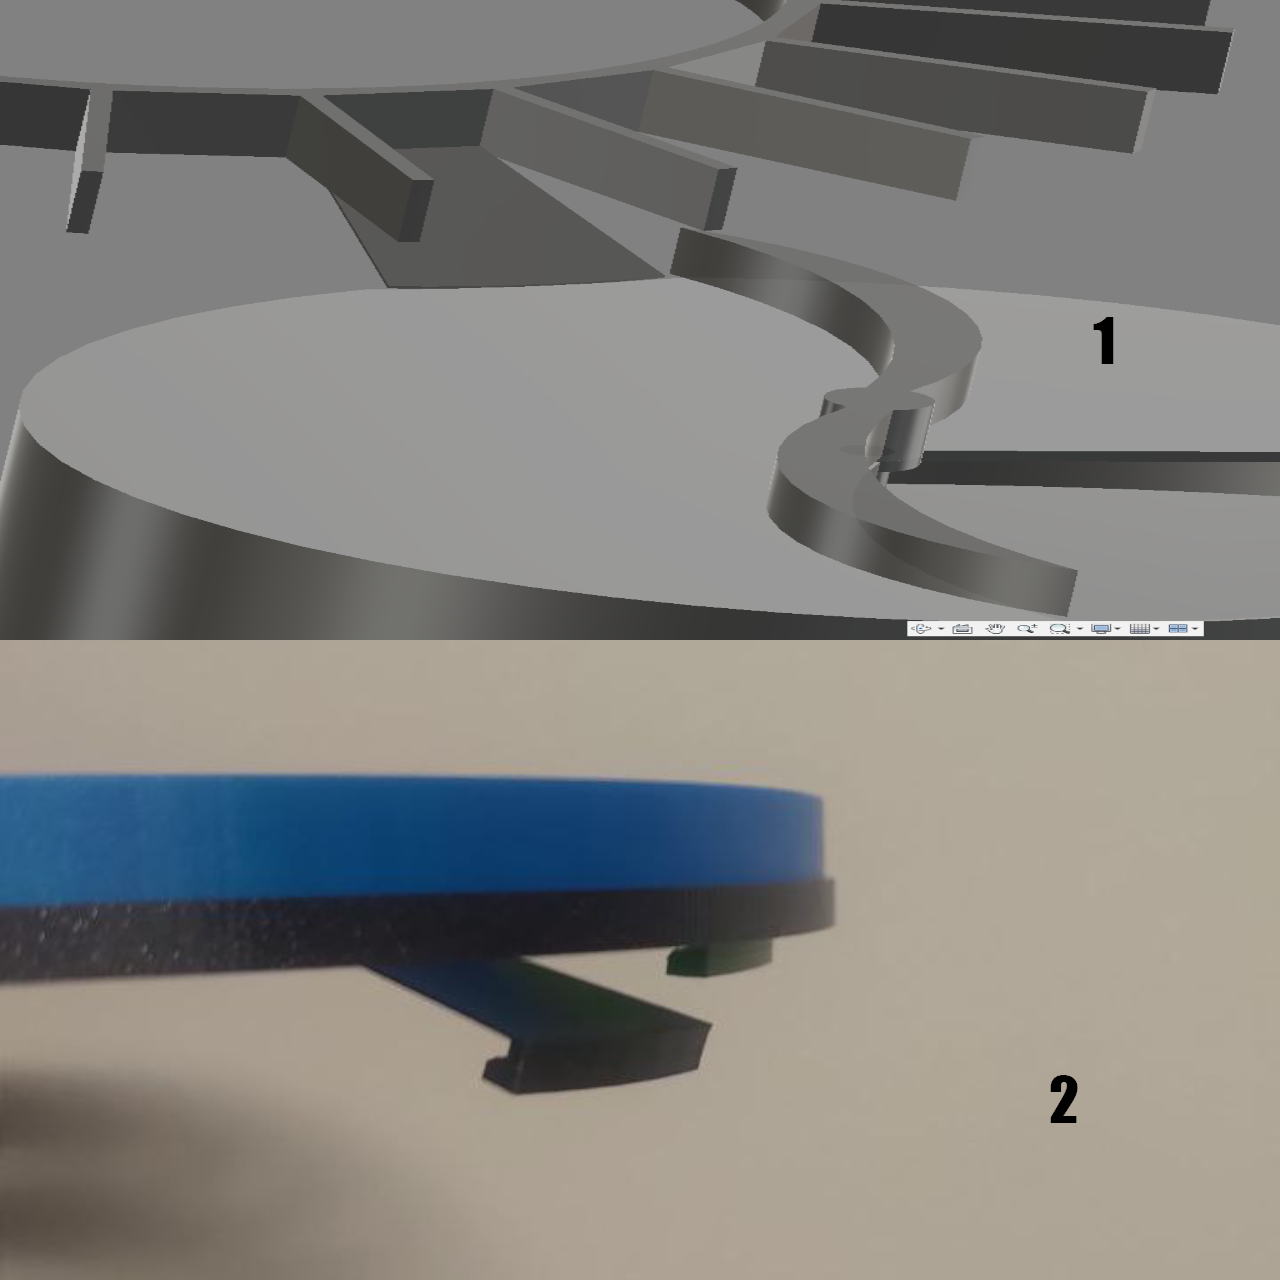
\includegraphics[width=0.7\linewidth]{Figures/Untitled-2}
	\caption[First revolver prototype]{First revolver prototype. Here you can see that initial idea was to have a trapdoor in each chamber which will release the pills onto the disposal dish by opening it.}
	\label{fig:screenshot1}
\end{figure}
\newpage
\subsubsection{Redesigning the Revolver System. A new approach}
Having realized that we need to get rid of the extra space that the separate body at the side of the main body takes, the new approach was required. This time, the disposal chambers would be directly underneath the dispensing chambers and we would use the power of gravity to move from one chamber to another, as you can see in the image \ref{fig:pspd2}. This would drastically reduce the amount of space the pill dispenser takes, singnificantly reduce complexity, setting all the rotating objects onto a single axis.


\begin{figure}[h]
	\centering
	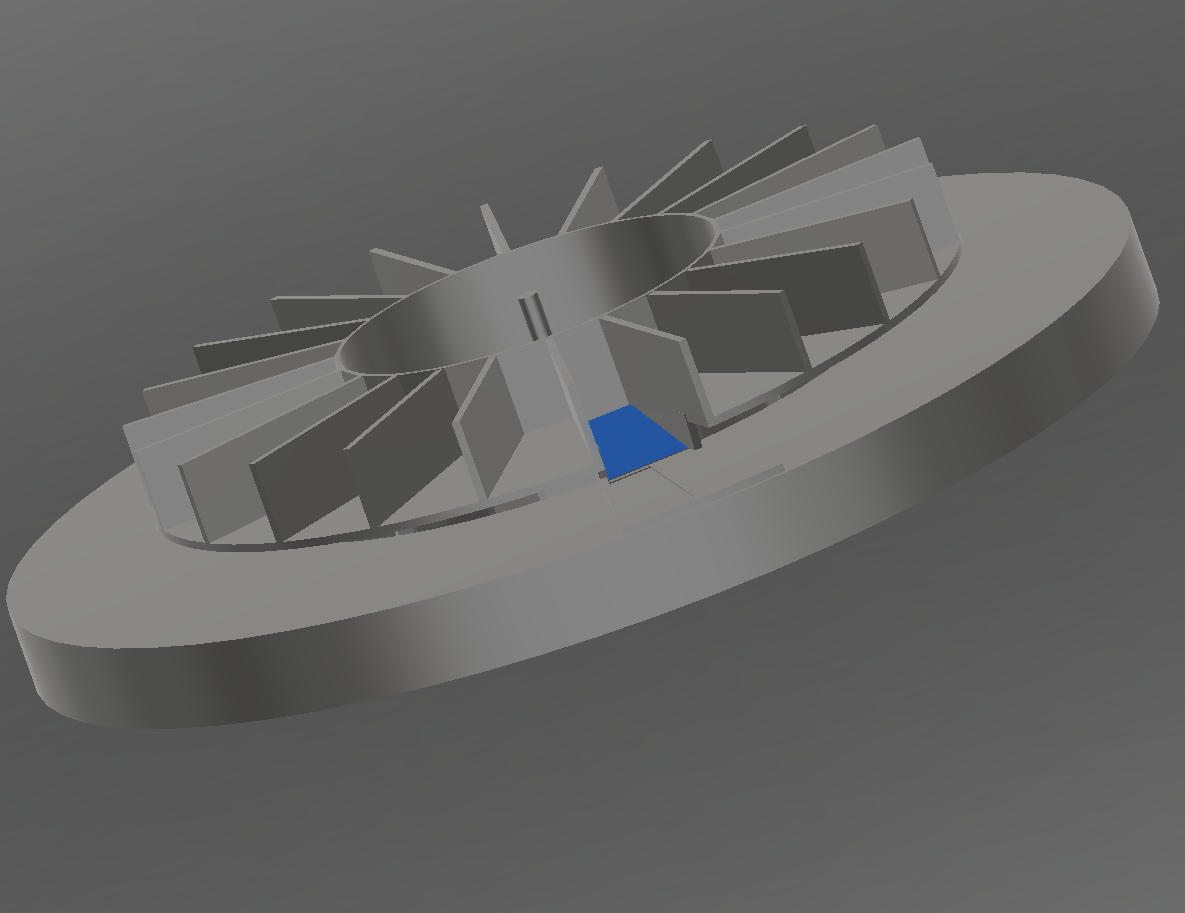
\includegraphics[width=0.7\linewidth]{Figures/PSPD2}
	\caption[2 Variante des Pillenspenders.]{2 Variante des Pillenspenders.}
	\label{fig:pspd2}
\end{figure}

Because this system doesn't have a separate mechanism for removing unused pills, another new method would have to be developed for this too. In the image \ref{fig:screenshot2} you can see how the chambers of the disposal system look like. The cover of the disposal system has an opening (part 2 of the same image) that is shut when the pills have to be taken. When the upper mechanism rotates to dispose new pills, the lower mechanism rotates to send pills into disposal chamber simultaneously. Ridges are added to the cover of disposal system to prevent pills from accidentally rolling away.

\begin{figure}
	\centering
	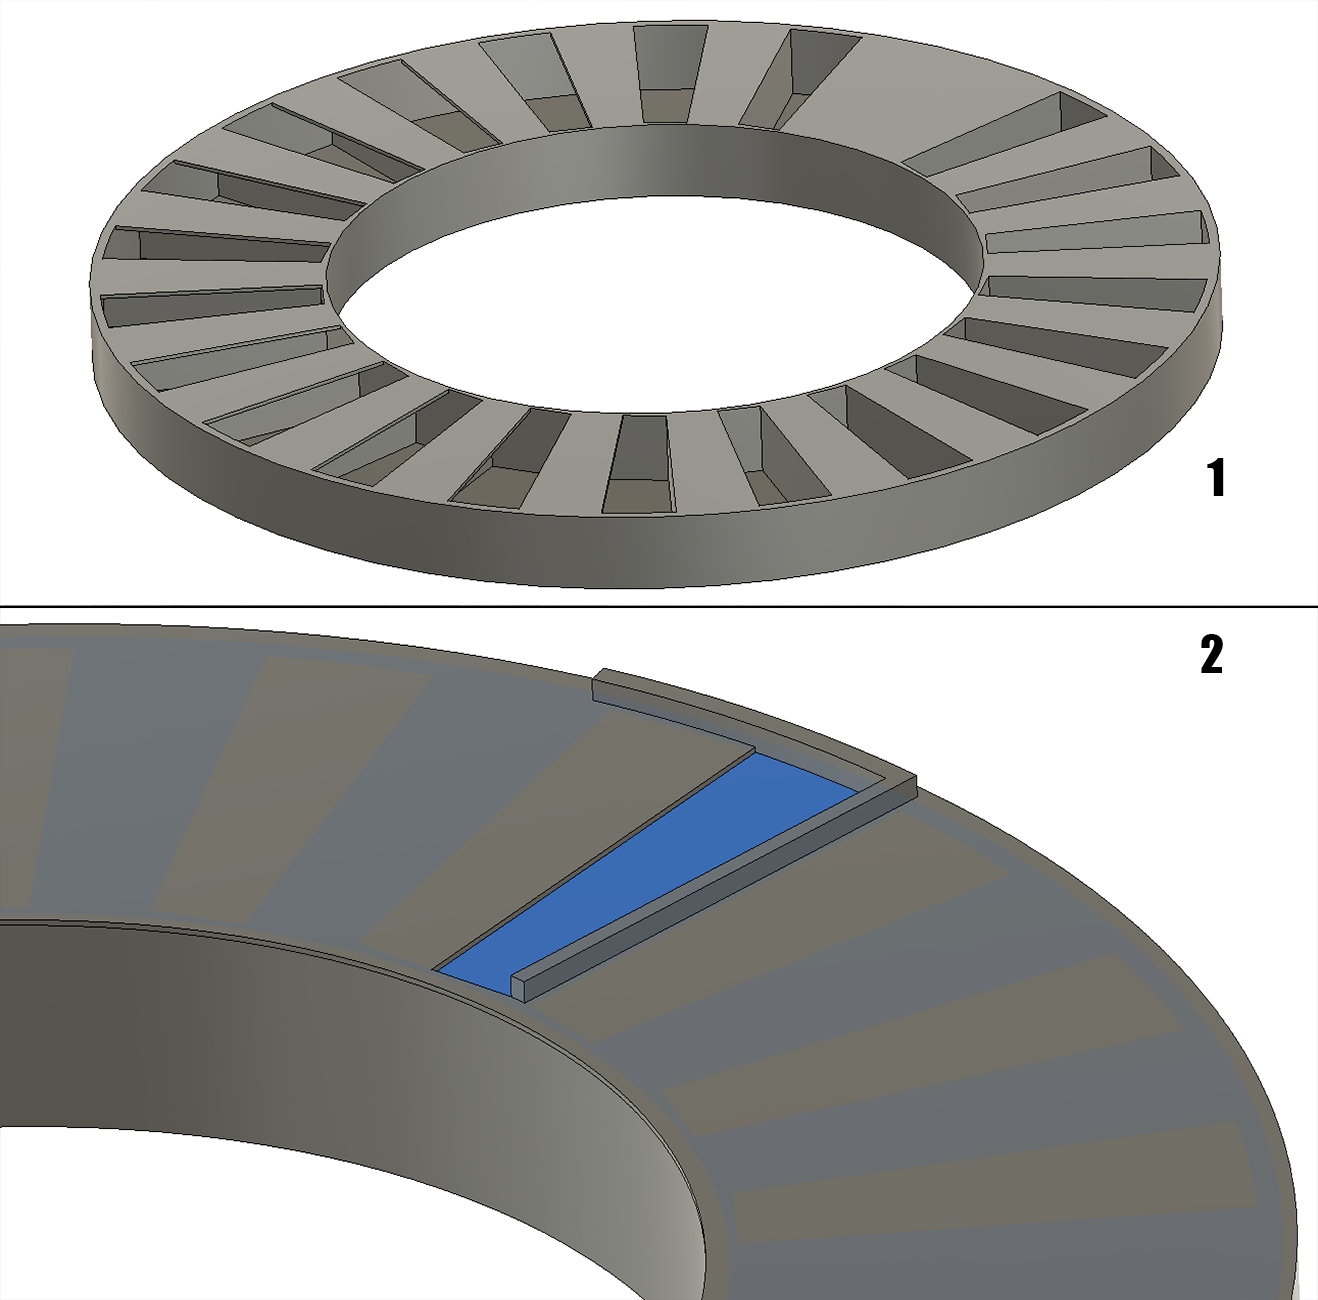
\includegraphics[width=0.7\linewidth]{Figures/PSPD2-Chambers}
	\caption[Disposal system of 2nd revolver system]{Disposal system of 2nd revolver system}
	\label{fig:screenshot2}
\end{figure}
\newpage
However, there are still ways to improve this approach. While much better than the previous one, this one also have some disadvantages:
\begin{enumerate}
\item \textbf{Chambers of the upper mechanism are smaller.} The chambers of pill storage are significantly smaller. We can calculate chamber volume using the following formulas:
\[
A = \pi r_1^2 - \pi r_0^2,\quad V = A \cdot h
\]
For the upper chamber: \( r_1 = 100\,\text{mm} \),\( r_0 = 47.5\,\text{mm} \), \( h = 18\,\text{mm} \), the result is:
\[
V = 437.90\,\text{cm}^3
\]
For the lower chamber:  \( r_1 = 135\,\text{mm} \), \( r_0 = 80\,\text{mm} \), \( h = 18\,\text{mm} \), the result is:
\[
V = 668.69\,\text{cm}^3
\]
As we can see, the lower chambers are almost 1.5 bigger than the upper ones, which is a waste that we might want to get rid of.
	\item{\textbf{Synchronous movement of both chambers}} This approach makes future development less flexible. independence of the chambers is a degree of freedom that we might want to keep somehow. The biggest problem with current approach is that it might lead to situations where some pills might fall too fast from the top to fall directly into an opening in time.
	\item{\textbf{Reliance on a ramp for pills to fall down.}} This can introduce an undesired behavior where some sticky pills might stick to the ramp and not fall down. This can lead to very dangerous scenario where a pill, not properly dispenced in time, would fall down with the next batch which would then lead to overdose.
\end{enumerate}

As mentioned earlier, this design is already what we would like to see as a final result, but we can improve it further, by redesigning it a bit and adressing the disadvantages we mentioned above.
\newpage

\subsubsection{The final redesign. Improving on what's good.}
A few thoughts come to mind as a potential approach to the redesign. Using gravity is obviosly good, we need to continue doing, however we might change how we use it. Having 2 systems one above another is also a great idea, what if we can make the chambers the same size? We could reposition the holes. Regarding synchronous movement, we have 2 types of direction of pill movement: From dispense to patient (intended behavior) and from dispense to disposal (backup behavior). The intended behavior implies human interaction, we can make some simple movement to deliver pills that would remove the need for synchronicity from our system. All these ideas are implemented in the final design, however it is worth mentioning that there has also been the intermediary step, where the dispense mechanism was rotated 90 degrees (see image \ref{fig:screenshot4}), so that it is completely vertical. It is worth giving a short overview of why this idea wasn't chosen as final:
\begin{itemize}
	\item{\textbf{Too tall}} the wheel with diameter of 100mm would be vertically positioned which takes a lot of space.
	\item{\textbf{Requires more Rotational momentum}} A motor would have to directly resist the force of gravity to lift the pills up a mill
	\item{\textbf{Doesn't fix synchronicity}} The mechanisms are still locked together, this issue remains unresolved.
\end{itemize}
\begin{figure}[]
	\centering
	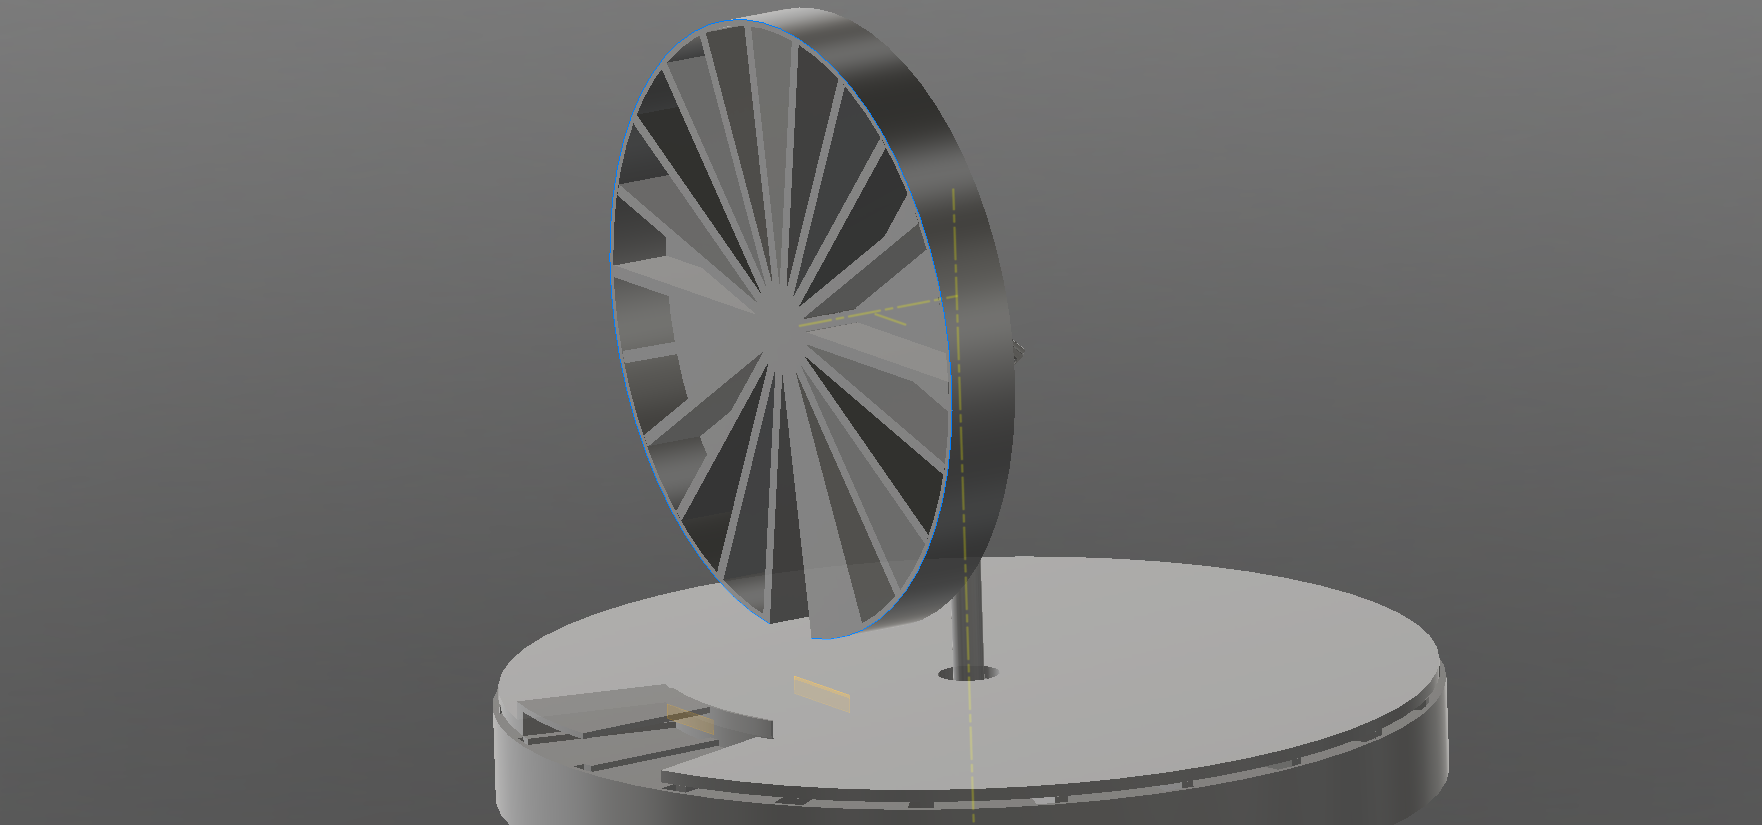
\includegraphics[width=0.6\linewidth]{Figures/Screenshot_4}
	\caption[Vertical Pillenspender.]{Pill dispenser with dispense system rotated vertically.}
	\label{fig:screenshot4}
\end{figure}
\newpage
For the final design, the following steps have been taken to address the issue:
\begin{enumerate}
	\item{\textbf{Resize the chambers}} Chambers size were changed so that they match. The result is device now has a cylindircal form where the chamber mechanisms are located directly on top of each other, maximising the space used
	\item{\textbf{Remove the ramp, change disposal mechanism}} The disposal mechanism was also changed. It works in tandem with dispense mechanism, which was also changed. The pills are now dispensed by the same movement by which they are made available, namely by rotation of the dispense mill. 
	\item{\textbf{Introduce a separate axis of rotation to dispense pills}} We will use tilting movement of the whole device for dispense of the pills into a cup or a hand of a patient, but for that we would nave the whole construction elevated.
	\item{\textbf{Exapnd the device to include the stand}} As mentioned above, it needs to be elevated. The stand will provide not only the elevation, but also another axis of rotation, therefore decoupling the disposal and dispense mechanisms from one another.
\end{enumerate}
In the image \ref{fig:screenshot5} you can see the final design. It has all the features mentioned above already covered. In the next chapter we will go step by step into the details of the design and see how the proposed soultions were implemented.
\begin{figure}[]
	\centering
	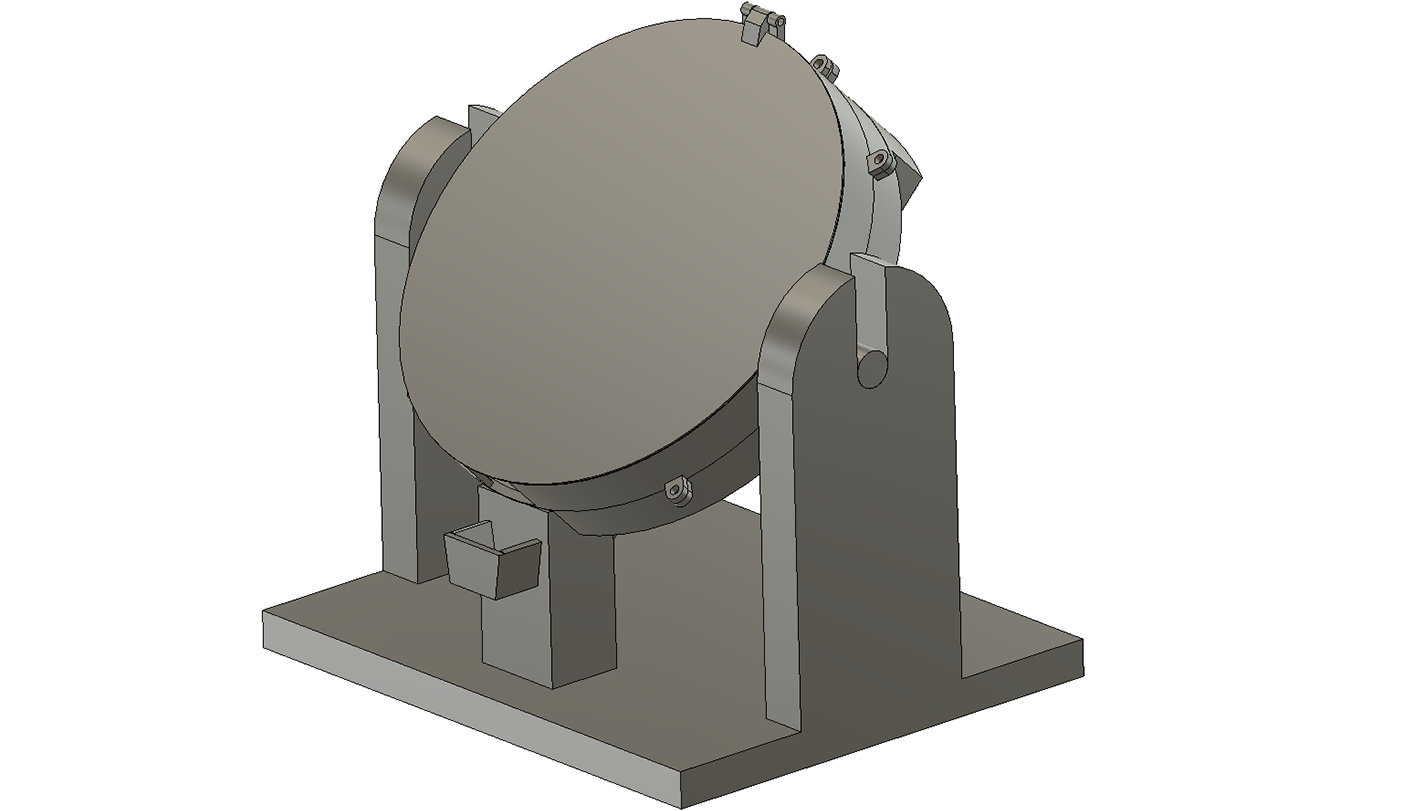
\includegraphics[width=0.6\linewidth]{Figures/Screenshot_5}
	\caption[Final result]{The final design of the Pillenspender.}
	\label{fig:screenshot5}
\end{figure}


